\begin{wrapfigure}{r}{0.27\textwidth}
  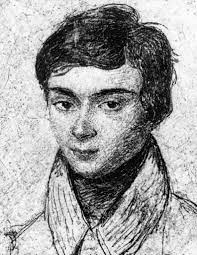
\includegraphics[scale=0.7]{galois.jpg}
  \caption{Galois}
\end{wrapfigure}

Galois Theory is a popular and one of the important theory in Abstract Algebra. It's foundation was first laid by the French Mathematician \textit{Évariste Galois} by determining the necessary and sufficient condition for solving the polynomial equation by radicals and thereby solving the problem that was open for 350 years old.\\ \\
The core-part of the Galois Theory is the \textit{Fundamental Theorem} of Galois Theory which links two main parts of Abstract Algebra; Field Theory and Group Theory. This is a profound result in Abstract Algebra. \\

\section{Approaches to the Theory}
\begin{enumerate}
\item Galois approached this problem by using the group of permutations of the roots of a polynomial equation. Only those permutations of the roots are considered which leaves any equation satisfied by the roots unchanged.

\item The modern approach is to use the \textbf{field extension} of the underlying field of the polynomial and examine the groups of automorphism of the extension field that fixes the underlying field.
\end{enumerate}
\clearpage

\section{Structure of a Field Extension}
Let \(F=K(u)\) be a field extension of the field \(K\). Then \(F\) is a vector space over \(K\) generated by \(u\).\\
We have \(u^n \in F\) for all \(n \in \mathbb{Z}\) because F is a field. As \(F\) is a vector space over \(K\); \(F\) consists of all linear combinations of \(u^n \)'s, and the quotients of these linear combinations. A such linear combinations is: \(a_nu^n+a_{n-1}u^{n-1}+...+a_1u+a_0\) which is  given by the polynomial \(f(u)\), where \(f(x)=a_nx^n+a_{n-1}x^{n-1}+...+a_1x+a_0\).\\

So the structure of the extension field \(F=K(u)\) is:\\
\(F= \{\frac{f(u)}{g(u)} \;| \; f,g \in K[x],g(u) \neq 0\}\).\\

\begin{theorem}[Existence of an Extension field]
If K is a field and \(f \in K[x]\) is a polynomial of degree \(n\),then there exists a simple extension field \(F=K(u)\) of K such that \(u\in F\) is a root of \(f\).~\cite{hunger}
\end{theorem}

\section{Algebraic and Transcendental element}
\begin{theorem}
Let \(F\) be an extension field of a field \(F\).\\
A map \(\phi:K[X] \rightarrow K[u]\) where \(u \in F\) defined by \(\phi (f(x))=f(u)\)\\
i.e, \(\phi (a_0+a_1x+...+a_nx^n)= a_0+a_1u+...+a_nu^n\) is a ring homomorphism.
\end{theorem}

Thus \( K[x]\) and \(K[u]\) are homomorphic.
  \begin{enumerate}
  \item If \(u\) is transcendental over \(K\) then \(K[u]\) is not a field and \(K[x] \cong K[u]\).
  \item If \(u\) is algebraic over \(K\) then, \(K[x] \ncong K[u]\) because \(Ker\phi\) is non trival and we have,
    \begin{enumerate}
    \item[i)] \(K(u) \cong K[u]\);
    \item[ii)] \(K(u) \cong K[x]/(f)\), where \(f \in K[x]\) is an 'irreducible monic polynomial of degree \(n \geq 1\);
    \item[iii)] \([K(u):K]=n\) and \(\{1_k,u,u^2,...,u^{n-1}\}\) is a basis of the vector space \(K(u)\) over \(K\).
    \end{enumerate}
  \end{enumerate}

\begin{theorem}[Isomorphism of Extension fields]
 Let K be a field.\\
 Then 'u' and 'v' are  roots of the same irreducible polynomial \(f \in K[x]\) if and only if there is an isomorphism of fields \(K[u] \cong K[v]\) which sends u onto v and is the identity on \(K\).
\end{theorem}



%%% Local Variables:
%%% mode: latex
%%% TeX-master: "n"
%%% End:
